% Artículo: predicción de llegadas de autobús con feeds que solo dan la posición y horarios interpolados.
% Compilar con: latexmk -pdf articulo.tex (pdflatex + biber). Las cifras de las tablas salen de resultados.py.
\documentclass[preprint,11pt,nonatbib]{elsarticle}

\usepackage[T1]{fontenc}
\usepackage[utf8]{inputenc}
\usepackage{lmodern}
\usepackage{microtype}
\usepackage{amsmath,amssymb,amsthm}
\usepackage{booktabs,tabularx}
\usepackage{xcolor}
\usepackage{tikz}
\usetikzlibrary{arrows.meta,positioning,decorations.pathreplacing}
\usepackage{pgfplots}
\pgfplotsset{compat=1.18}
\usepackage{algorithm}
\usepackage{algpseudocode}
\usepackage[hidelinks]{hyperref}
\makeatletter\let\c@author\relax\makeatother
\usepackage[style=authoryear,backend=biber,maxcitenames=2,uniquelist=false,giveninits=true,doi=true,url=false]{biblatex}
\addbibresource{referencias.bib}

\definecolor{ruta}{HTML}{01573C}
\definecolor{gps}{HTML}{C8102E}
\definecolor{gris}{HTML}{6B7280}

% Notación (la de la memoria técnica).
\newcommand{\Tpos}{T_{\mathrm{pos}}}
\newcommand{\tgps}{t_{\mathrm{gps}}}
\newcommand{\tref}{t_{\mathrm{ref}}}
\newcommand{\ETA}{\mathrm{ETA}}
\newcommand{\band}{\operatorname{band}}
\newcommand{\clamp}{\operatorname{clamp}}
\newcommand{\med}{\operatorname{med}}

% Pie de la primera página: preprint, versión y fecha (en lugar de «Preprint submitted to Elsevier»).
\makeatletter
\def\ps@pprintTitle{%
  \let\@oddhead\@empty
  \let\@evenhead\@empty
  \def\@oddfoot{\footnotesize\itshape Preprint, version 0.1 \hfill \today}%
  \let\@evenfoot\@oddfoot}
\makeatother

\newtheorem{definition}{Definition}

\begin{document}

\begin{frontmatter}

\title{Predicting bus arrivals when the feed reports positions but not delays: a reproducible three-layer method
with an open reference implementation}

\author{Yeray Garrido\fnref{orcid}}
\fntext[orcid]{Independent researcher, Bilbao, Biscay, Spain. ORCID:
\href{https://orcid.org/0009-0008-0459-0294}{0009-0008-0459-0294}. Contact through
\url{https://github.com/Garridoparrayeray/bide-eta}.}

\begin{abstract}
Many public transport networks publish the position of their vehicles in real time but not their delay, and many
timetables give intermediate stop times interpolated at constant speed rather than observed. Bizkaibus, the
interurban bus network of Biscay (Spain), has both properties: after the first hour of a trip, 85\% of buses pass a
stop more than two minutes before the published time. This paper describes, in enough detail to be reimplemented in
any language, the arrival prediction method of the Bizkaibus+ app. The method works with timetable differences
instead of absolute times, learns the actual travel time of every segment between consecutive stops by time band
with medians shrunk towards the all-day median of the segment, and predicts in three layers with explicit
abstention rules: the vehicle position projected on the route, the last stop registered by the feed, and the
timetable corrected trip by trip. It recalibrates itself every day and only adopts changes that reduce the error
measured on held-out days. On 9.1 million predictions over 23 days checked against the actual passage, the displayed
arrival is within $\pm2$~minutes in 92--96\% of cases when the bus is less than three minutes away and in 67\% at
ten to twenty minutes, against 23--25\% for the published timetable. Without any live data, the corrected timetable
alone doubles the accuracy of the published one. A reference implementation in Python, 323 test vectors produced by
the production engine, a public evaluator that reproduces the production evaluation exactly, and the learned tables
and evaluation data are openly available.
\end{abstract}

\begin{keyword}
bus arrival prediction \sep real-time passenger information \sep GTFS \sep SIRI \sep robust estimation \sep
shrinkage \sep temporal validation \sep reproducibility
\end{keyword}

\end{frontmatter}

% =====================================================================================================================
\section{Introduction}
\label{sec:intro}

Real-time arrival information reduces the time passengers wait at stops and the uncertainty of the wait, and makes
public transport more attractive \parencite{watkins2011,brakewood2019}. Producing it requires two inputs that are not
always available in the form a prediction method expects: a reliable reference schedule and a live estimate of how
far each vehicle is from it.

Bizkaibus, the interurban bus network of the province of Biscay in northern Spain, publishes both through open
data: a GTFS timetable \parencite{gtfs} and a SIRI Vehicle Monitoring feed \parencite{siri} with the GPS position and
the next stop of every vehicle in service. The feed, however, does not carry the delay of the vehicle, and the
intermediate times of the timetable are not commitments of the operator: they are a linear interpolation between
the times of the terminals, at constant speed along the route. The real bus is slower in towns and faster on
highways, so the published intermediate times drift away from the real passages as the trip advances.
Section~\ref{sec:data} quantifies the drift: over 169,308 observed stop passages, after the first hour of a trip 85\%
of buses pass more than two minutes before the published time, with a median of almost fourteen minutes early. A
passenger who trusted the published time and reached the stop two minutes early would find that the bus had already
gone in 52\% of cases.

The setting is not specific to Bizkaibus. Position-only feeds are common in automatic vehicle location systems, and
interpolated intermediate times are allowed by GTFS (\texttt{timepoint=0}) and widespread in regional networks. Under
these conditions, the absolute published time is a poor reference, and a method that predicts arrivals by adding a
delay to it inherits its error.

This paper describes the method that the Bizkaibus+ app\footnote{\url{https://www.bideplus.eus}. The app is
independent and has no relation with Bizkaibus, the Diputación Foral de Bizkaia or the operators of the service.}
uses to predict arrivals under these conditions. Its purpose is to make the method reusable: every rule is given with
its formula and constants, the evaluation protocol is specified so that it can be repeated on other data, and the
reference implementation, test vectors, evaluator and data are public. The contributions are:

\begin{enumerate}
  \item A representation of the vehicle state in \emph{timetable time}: the GPS position is projected on the route
        and converted into the scheduled time at that point, so that predictions are built from timetable
        differences, which are reliable even when absolute times are not (Section~\ref{sec:method}).
  \item A segment travel-time model learned from the feed itself, by time band and day type, with medians shrunk
        towards the all-day median of each segment, and a daily recalibration that only adopts changes that reduce
        the error on held-out days.
  \item A three-layer prediction with explicit abstention rules, which decides for every stop whether the vehicle
        position, the last registered stop or the corrected timetable gives the best available estimate, and says so.
  \item An open, verifiable package: a reference implementation written only from the specification, 323 test
        vectors produced by the production engine, an evaluator that reproduces the production histograms bin by
        bin, and the learned tables and evaluation data (Section~\ref{sec:reuse}).
\end{enumerate}

\noindent The rest of the paper reviews related work (Section~\ref{sec:related}), describes the data and the problem
(Section~\ref{sec:data}), the method (Section~\ref{sec:method}) and the evaluation (Section~\ref{sec:evaluation}),
explains how to reproduce and reuse the results (Section~\ref{sec:reuse}), discusses limitations and open problems
(Section~\ref{sec:discussion}) and concludes (Section~\ref{sec:conclusions}).

\begin{figure}[t]
\centering
\fbox{\begin{minipage}{0.94\textwidth}\small
\textbf{The method in plain words.} The timetable says, for every stop, when the bus should pass; its intermediate
times are wrong in absolute terms but consistent with each other. The method first asks \emph{where in the timetable}
the bus is: it projects the GPS position on the route and reads the scheduled time at that point. A bus that is
physically where the timetable puts it at 10:20 is, in timetable terms, at 10:20, whatever the clock says. To predict
the arrival at a later stop, it does not add a delay to the published time of that stop; it adds, to the current
clock time, how long the remaining segments \emph{actually} take, learned from weeks of observed passages. When the
GPS is missing or unreliable, it uses the last stop the feed says the bus passed; when there is no live data at all,
it uses the timetable corrected with what each trip usually does. Each prediction says which of these three it is.
\end{minipage}}
\end{figure}

% =====================================================================================================================
\section{Related work}
\label{sec:related}

% Se completa con la bibliografía verificada (related-work.bib): revisiones, métodos por tramos e históricos,
% filtros de Kalman, aprendizaje automático, estudios con GTFS-Realtime y calidad de los feeds, contracción.

Bus arrival time prediction has been studied with historical averages and regression, Kalman filters, artificial
neural networks and, more recently, deep learning models. Early work used neural networks trained on automatic
vehicle location data \parencite{chien2002} and combined them with Kalman filters to update predictions with the
latest observations \parencite{shalaby2004}. Kalman filtering \parencite{kalman1960} remains a common baseline for
the delay of a single vehicle. The relationship between published schedules, observed running times and the
uncertainty of predictions has also been studied from the passenger's side
\parencite{mishalani2006,watkins2011,brakewood2019}.

% =====================================================================================================================
\section{Data and problem setting}
\label{sec:data}

\subsection{Timetable}
The timetable is the GTFS feed of Bizkaibus published through the Spanish National Access Point for transport
\parencite{nap}. It contains about 100 lines. Every line has an identifier (\texttt{route\_id}, e.g.\ \texttt{651})
and a public name (\texttt{route\_short\_name}, e.g.\ \texttt{A0651}). Intermediate stops carry
\texttt{timepoint=0}: their times are interpolated linearly in distance between the times of the terminals.

\subsection{Live feed}
The SIRI Vehicle Monitoring feed is a public XML document regenerated about once a minute, with about 250 vehicles at
peak hours. For every vehicle it gives the trip reference (equal to a GTFS \texttt{trip\_id}), the vehicle
identifier, the GPS position and its time, and the order of the next stop of the trip. It does not give the delay.
From 23:58 to 05:00 the feed repeats the vehicles seen before midnight with their old times; those entries carry no
time of the new day and are ignored (Section~\ref{sec:method}).

\subsection{Why the timetable is not an absolute reference}
\label{sec:drift}

Figure~\ref{fig:drift} shows the deviation between the actual passage and the published time over 169,308 observed
stop passages, as a function of the scheduled time elapsed since the departure from the terminal. Near the terminal
buses are slightly late (median $+1.3$~min in the first ten minutes). From there on they are increasingly early: at
half an hour from the departure, half of the passages happen more than two minutes before the published time, and
after one hour 85\% do, with a median of almost fourteen minutes early. Only a quarter of all passages fall within
$\pm2$~minutes of the published time. These figures are not a judgement on the punctuality of the service, since the
intermediate times are not commitments of the operator; they are, however, the times that a passenger sees in any
application that does not correct them.

\begin{figure}[t]
\centering
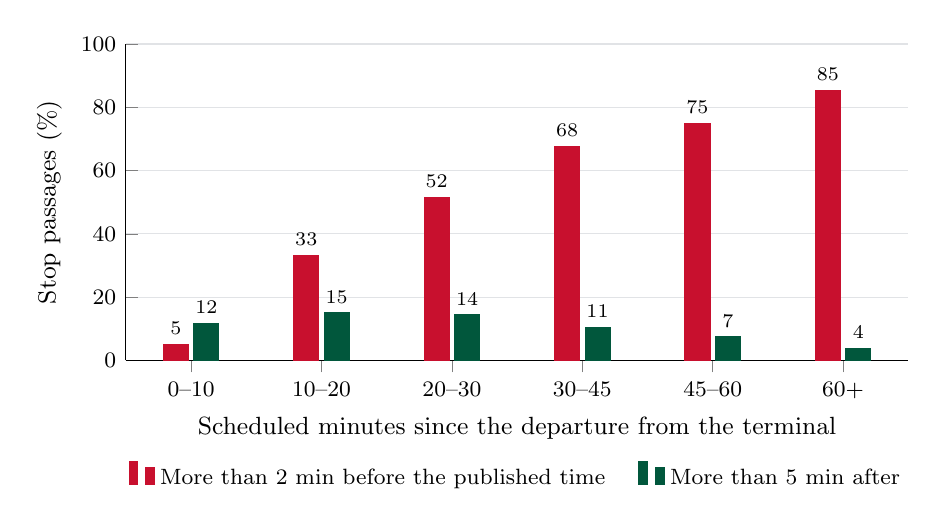
\begin{tikzpicture}
\begin{axis}[
  width=0.95\textwidth, height=5.6cm,
  ybar, bar width=9pt,
  symbolic x coords={0--10,10--20,20--30,30--45,45--60,60+},
  xtick=data,
  xlabel={Scheduled minutes since the departure from the terminal},
  ylabel={Stop passages (\%)},
  ymin=0, ymax=100,
  axis lines*=left, ymajorgrids, grid style={gris!20},
  tick label style={font=\footnotesize}, label style={font=\small},
  legend style={font=\footnotesize,draw=none,fill=none,at={(0.5,-0.3)},anchor=north,legend columns=2,/tikz/every even column/.append style={column sep=1em}},
  nodes near coords, every node near coord/.append style={font=\scriptsize,color=black},
  nodes near coords style={/pgf/number format/fixed,/pgf/number format/precision=0}]
\addplot[fill=gps,draw=gps] coordinates {(0--10,5.0) (10--20,33.3) (20--30,51.5) (30--45,67.6) (45--60,74.8) (60+,85.4)};
\addlegendentry{More than 2 min before the published time}
\addplot[fill=ruta,draw=ruta] coordinates {(0--10,11.8) (10--20,15.0) (20--30,14.4) (30--45,10.5) (45--60,7.4) (60+,3.7)};
\addlegendentry{More than 5 min after}
\end{axis}
\end{tikzpicture}
\caption{Deviation of the actual passage from the published time, by scheduled time since the departure (169,308
stop passages). Because the timetable spreads time at constant speed and buses run faster on the road sections, they
pass increasingly early as the trip advances.}
\label{fig:drift}
\end{figure}

% =====================================================================================================================
\section{Method}
\label{sec:method}

% PENDIENTE: se escribe a partir de la lectura completa de los capítulos 4 a 7 de la memoria (localización, modelo,
% predicción en tres capas, aprendizaje), con las fórmulas, las constantes y el pseudocódigo.

% =====================================================================================================================
\section{Evaluation}
\label{sec:evaluation}

\subsection{Protocol}
\label{sec:protocol}

The evaluation replays captures of the live feed: snapshots taken every 20~s and stored in one-hour blocks. In each
snapshot, for every vehicle and every stop from its declared next stop $n$ to $n+8$, the method predicts the arrival
$t_{\mathrm{shown}}$ that a user would see, and the published time $a$ is kept for comparison. The error is
\begin{equation}
e=\frac{t_{\mathrm{shown}}-t_{\mathrm{actual}}}{60}\ \text{minutes},
\end{equation}
positive when the bus arrives before the time shown.

\paragraph{Ground truth} The feed has no passage events, so the actual passage is reconstructed from the change of the
next stop: if in snapshot $m$ a vehicle that has stayed on the same trip declares for the first time a next stop
later than $q$, it passed stop $q$ between snapshots $m-1$ and $m$, and
\begin{equation}
t_{\mathrm{actual}}=\frac{t_{m-1}+t_m}{2},
\end{equation}
where $t_m$ is the most recent position time in snapshot $m$. The resolution is half the interval between
snapshots, and the measured error includes it. This reconstruction does not use the GPS, and is therefore independent
of the projection that the method itself uses.

\paragraph{Metrics} Predictions are grouped by horizon, the time that actually remained until the arrival (0--3,
3--6, 6--10 and 10--20 minutes), because accuracy depends mostly on it. The main metric is the share of predictions
within $\pm1$, $\pm2$ and $\pm3$ minutes, which answers the passenger's question (``will I make it if I leave when it
says?'') and is not dominated by a few large errors as the mean squared error would be. Errors are stored as
histograms of 15-second bins, so that any figure can be recomputed by adding captures.

\paragraph{Modes} Besides the full method, two ablations replay the same captures: \emph{without GPS}, where all
positions are deleted and only the stop registered by the feed remains, and \emph{without feed}, where the method
sees no live data and can only use the corrected timetable.

\paragraph{Data} Two consecutive periods are evaluated. From 15 to 31 October 2026 the evaluation kept summaries per
capture block (17 days with predictions, 2.21 million predictions within 20 minutes). From 31 October to 6 November
it kept the full histograms (7 days, 6.87 million predictions within 20 minutes in each mode), and the raw captures
are archived, so that this period can be re-evaluated with any version of the method. The method was updated during
both periods; the figures describe it as it ran in production.

\subsection{Results}

Table~\ref{tab:horizons} gives the accuracy by horizon. In both periods the arrival shown is within $\pm2$~minutes in
92--96\% of cases below three minutes and in 67\% between ten and twenty minutes, while the published timetable
stays at 23--25\% at every horizon. The median absolute error grows from 30~s below three minutes to 90~s at ten to
twenty minutes (second period, at the 15-second resolution of the histograms).

\begin{table}[t]
\centering
\caption{Share of arrivals within $\pm1$, $\pm2$ and $\pm3$ minutes of the actual passage, by horizon.}
\label{tab:horizons}
\small
\begin{tabular}{@{}lrrrrrrr@{}}
\toprule
& & \multicolumn{3}{c}{Method} & \multicolumn{3}{c}{Published timetable} \\
\cmidrule(lr){3-5}\cmidrule(l){6-8}
Horizon (min) & Predictions & $\pm1$ & $\pm2$ & $\pm3$ & $\pm1$ & $\pm2$ & $\pm3$ \\
\midrule
\multicolumn{8}{@{}l}{\emph{15--31 October 2026 (17 days)}} \\
0--3   & 534,046 & 84 & 96 & 98 & 13 & 24 & 34 \\
3--6   & 485,601 & 67 & 90 & 96 & 13 & 24 & 34 \\
6--10  & 548,058 & 53 & 82 & 92 & 12 & 23 & 33 \\
10--20 & 640,763 & 39 & 67 & 82 & 13 & 25 & 35 \\
\midrule
\multicolumn{8}{@{}l}{\emph{31 October--6 November 2026 (7 days)}} \\
0--3   & 1,485,997 & 81 & 92 & 94 & 12 & 23 & 33 \\
3--6   & 1,371,035 & 67 & 89 & 95 & 13 & 24 & 34 \\
6--10  & 1,673,835 & 54 & 82 & 92 & 12 & 23 & 33 \\
10--20 & 2,339,535 & 39 & 67 & 82 & 13 & 25 & 35 \\
\bottomrule
\end{tabular}
\end{table}

\paragraph{What each source of information contributes} Table~\ref{tab:ablation} compares the full method with the two
ablations on the second period. Deleting the GPS costs little: the stop registered by the feed is updated often
enough that, below three minutes, accuracy is the same, and at ten to twenty minutes it drops from 67\% to 64\%.
Without any live data, the corrected timetable reaches 50--54\% within $\pm2$~minutes at every horizon, twice the
published timetable: half of the gain comes from learning how long the segments really take, before any live data is
used.

\begin{table}[t]
\centering
\caption{Share of arrivals within $\pm2$ minutes with all the information, without GPS positions and without any
live data (31 October--6 November 2026).}
\label{tab:ablation}
\small
\begin{tabular}{@{}lrrrr@{}}
\toprule
Horizon (min) & Full method & Without GPS & Without feed & Published timetable \\
\midrule
0--3   & 92 & 93 & 50 & 23 \\
3--6   & 89 & 87 & 54 & 24 \\
6--10  & 82 & 79 & 53 & 23 \\
10--20 & 67 & 64 & 53 & 25 \\
\bottomrule
\end{tabular}
\end{table}

\paragraph{By layer} In the second period the first layer (GPS position) produced 85--94\% of the predictions,
depending on the horizon, with 97\%, 92\%, 84\% and 68\% within $\pm2$~minutes from the shortest to the longest
horizon. The second layer (registered stop) produced about 3\% of the predictions, and the third (corrected
timetable) between 3\% and 13\%. Third-layer predictions at less than three minutes are rarely right (6\%): they
correspond to buses that should be arriving but send no usable data. This is why accuracy below three minutes is
lower in the second period than in the first.

\paragraph{By day type} Weekday and weekend accuracy are similar (92\% and 92\% below three minutes, 67\% and 65\% at
ten to twenty minutes).

% PENDIENTE: comparación con el filtro de Kalman y la red neuronal (memoria, capítulo 8), y evaluación por días de la
% contracción.

% =====================================================================================================================
\section{Reproducing and reusing the method}
\label{sec:reuse}

All the material needed to verify the results and to reuse the method is in the public repository
\url{https://github.com/Garridoparrayeray/bide-eta}, under the MIT licence for code and CC~BY~4.0 for text and data.

\begin{itemize}
  \item \texttt{referencia/referencia.py} implements the method in Python using only the standard library. It was
        written from the specification, not from the production code.
  \item \texttt{referencia/vectores.json} contains 323 test vectors: concrete inputs and the exact output of the
        production engine, covering the projection, the three layers, the segment model, the pace factor, the
        per-trip correction and their calibration. \texttt{comprobar.py} runs the reference implementation on all of
        them; it reproduces the 323 outputs.
  \item \texttt{referencia/evaluar.py} replays captures of the live feed and writes the same 15-second histograms as
        the production evaluation. On 40 minutes of the live feed of 7 November 2026 (92,686 predictions), its
        histograms are identical bin by bin to those of the production evaluator in the three modes.
  \item \texttt{datos/} holds the learned tables (segment times, pace factors and per-trip corrections) and the
        evaluation data behind every table of this paper; \texttt{articulo/resultados.py} recomputes them.
\end{itemize}

\noindent Three conventions must be kept when porting the method to another language: times are seconds since
midnight of the service day and may exceed 86,400; rounding sends halves away from zero; and medians are low medians,
the element $\lfloor p(n-1)\rfloor$ of the sorted values.

% =====================================================================================================================
\section{Discussion and limitations}
\label{sec:discussion}

% PENDIENTE: a partir del capítulo 9 de la memoria y de los resultados nuevos.

% =====================================================================================================================
\section{Conclusions}
\label{sec:conclusions}

% PENDIENTE.

\section*{Data and code availability}
The reference implementation, test vectors, evaluator, learned tables and evaluation data are available at
\url{https://github.com/Garridoparrayeray/bide-eta} (MIT licence for code, CC~BY~4.0 for text and data). The
timetable and the live feed are open data of their publishers. The production engine of the app is not public.

\printbibliography

\end{document}
